\documentclass[13pt]{article}

\title{Relazione 5: Analisi spettrale del Pendolo Caotico}
\author{Antonio Michele Miti}

\usepackage{amsmath}
\usepackage[utf8]{inputenc}
\usepackage[italian]{babel}
\usepackage{listings}
\usepackage{textcomp}
\usepackage{graphicx}
\usepackage{subfigure}
\usepackage{rotating}
\usepackage{caption}
\usepackage{latexsym}
\usepackage{epstopdf}
\usepackage{eepic,epic,eepicemu}
\usepackage{color}
\pagestyle{headings}
\definecolor{listinggray}{gray}{0.9}
\definecolor{lbcolor}{rgb}{0.95,0.95,0.95}
\lstset{
	backgroundcolor=\color{lbcolor},
	rulecolor=,
	language=C++,
        basicstyle=\scriptsize,
        upquote=true,
        aboveskip={1.5\baselineskip},
        columns=fixed,
        showstringspaces=false,
        extendedchars=true,
        breaklines=true,
        prebreak = \raisebox{0ex}[0ex][0ex]{\ensuremath{\hookleftarrow}},
        frame=single,
        showtabs=false,
        showspaces=false,
        showstringspaces=false,
        identifierstyle=\ttfamily,
        keywordstyle=\color[rgb]{0,0,1},
        commentstyle=\color[rgb]{0.133,0.545,0.133},
        stringstyle=\color[rgb]{0.627,0.126,0.941},
}
\addtolength{\hoffset}{-1.25cm}
\addtolength{\voffset}{-1.80cm}
\addtolength{\textwidth}{1cm}
\addtolength{\textheight}{3.80cm}
\newtheorem{legge}{Teorema}

\begin{document}
\maketitle
\begin{abstract}
Questo articolo tratta dell'implementazione dell'algoritmo per la Trasformata di Fourier in linguaggio C++ e come sfruttare tali metodi nell'analisi spettrale di funzioni in particolare le traiettorie del Pendolo non Lineare Smorzato in configurazioni prossime a quella caotica.
\end{abstract}

%\tableofcontents

\section{Introduzione}
La Trasformata di Fourier è operativamente una trasformata integrale la cui immagine su una generica funzione $h(t)$ è definita come:
	\begin{equation}
	\mathcal{F}\lbrace h(t) \rbrace (f) \doteq H(f) = \int_{-\infty}^{\infty} h(t) e^{2 \pi  i  f  t}\, \textrm{d} t
	\end{equation}
è tale per cui :
	\begin{equation}
	h(t) = \int_{-\infty}^{\infty} H(f) e^{-2 \pi  i  f  t}\, \textrm{d} f \doteq \bar{\mathcal{F}}\lbrace H(f) \rbrace (t)
	\end{equation}.

Questi operatori assumono un significato molto profondo quando vengono visti come endomorfismi sullo spazio di Hilbert $ \mathcal{L}^2$ delle funzioni a quadrato sommabile secondo Lebesgue.
In sostanza la trasformata di fourier di una funzione h(t) non è altro che la funzione che esprime le componenti della funzione h(t) sulla base continua delle onde piane $\lbrace e^{i \omega t} \rbrace_{\omega \in \mathcal{R}} $ al variare del parametro continuo $\omega = 2 \pi f$.

La funzione trasformata $H(f)$ è una funzione a valori complessi, il modulo quadrato della trasformata $\mid H(f) \mid ^{2}$ è detto \emph{"Power Spectrum"}, lo studio di questo andamento permette di trarre informazioni sulla funzione: ad esempio uno spettro discreto è caratteristico di comportamenti periodici mentre uno spettro non nullo su un intervallo esteso è un buon indice di comportamenti caotici.




\subsection{DFT}

In ambito computazionale si può avere a che fare unicamente con funzioni samplate.

In altre parole bisogna identificare un algoritmo che a partire da N punti noti della funzione h(t) determini un campionamento della funzione trasformata H(f) in almeno N punti.

Sia la funzione $h(t)$ da trasformare, samplata in $N$ punti ad intervalli regolari $\Delta$, quindi si definisce $h_{n}$ la sequenza dei valori samplati:
$$ h_{n} = h ( n \Delta ) \qquad n = 0, \ldots , N-1 \qquad .$$

L'intervallo di samplaggio $\Delta$ determina la cosiddetta \emph{Frequenza Critica di Nyquist}
	\begin{equation}
	f_{c} = \dfrac{1}{2 \Delta}
	\end{equation}
tale che:
\begin{legge}[Campionamento di Nyquist]

Hp:	\begin{itemize}
	\item[-] $h(t)$ continua e samplata ad intervalli $\Delta$
	\item[-] $H(f) = \mathcal{F}\lbrace h(t) \rbrace (f)$ è a banda limitata a frequenze minori di $f_{c}$ ovvero $$H(f) = 0 \qquad \forall \vert f \vert \geq f_{c}$$
	\end{itemize}

Th: $h(t)$ è univocamente definita dai campioni $h_{n}$:
\begin{equation}
h(t) = \Delta \sum_{n= - \infty}^{+ \infty} h_{n} \dfrac{\sin[2 \pi f_{c} (t - n \Delta)]}{\pi (t - n \Delta)}
\end{equation}
\end{legge}

La conseguenza principale di questo teorema è l'esistenza del fenomeno detto \emph{Aliasing}, tale per cui la trasformata di fourier di funzioni sottosamplate risulta disturbata.

In Sostanza si ha che tutte le componenti dello sviluppo spettarle della funzione a frequenze maggiori di $f_{c}$ vengono erroneamente traslate all'interno dell'intervallo di frequenza $(- f_{c} , f_{c})$.

Questo implica che per una funzione continua sufficientemente samplata, nel momento in cui viene stimata la traformata di Fourier a partire da un numero di campioni discreto, si assume implicitamente che la trasformata di fourier sia zero all'infuori del intervallo fissato dalla frequenza critica.

Per determinare se una funzione sia sufficientemente samplata  bisogna verificare che i termini spettrali tendano a zero al tendere di $f$ a $f_{C}$. Se così non fosse i valori successivi a fc che verrebbero erroneamente traslati all'interno dell'intervallo, darebbero un apporto non trascurabile.




\subsection{Trasformata di Fourier lenta}

E' il metodo più ovvio per stimare la trasformata di fourier per una funzione samplata in N punti.

Si definiscono $$ h_{k} \equiv h(t_{k}) \qquad t_{k} \equiv k \Delta \qquad k = 0,1, \ldots , N-1 $$

Con $ N$ punti di input, samplati a partire dal tempo 0, si è al massimo in grado di generare N punti indipendenti di output, quindi si cerca un sampling della trasformata di fourier nel intervallo critico $( - f_{c} , f_{c} ) $ per valori discreti della frequenza:
$$ f_{n} = \dfrac{n}{N \Delta} \qquad n = -\frac{N}{2} , \ldots , \frac{N}{2}$$
i due estremi dell'intervallo corrispondono ai valori della frequenza critica di Nyquist, avendo lo stesso valore della trasformata contano come un solo punto.

Non resta che approssimare l'integrale della formula (1) ad una somma discreta, la via più immediata è applicare il metodo dei rettangoli:

	\begin{equation}
	H(f_{n}) = \int_{-\infty}^{\infty} h(t) e^{2 \pi  i  f_{n}  t}\, \textrm{d} t \, \simeq 
	\sum_{k = 0}^{N - 1} h_{k} e^{2 \pi  i  f_{n}  t_{k}} \, \Delta = \Delta \sum_{k = 0}^{N - 1} h_{k} e^{2 \pi i \frac{k n}{N}} \, \equiv \Delta H_{n}
	\end{equation}

Ciò che si ottiene è una mappa da N valori complessi ( gli $h_{k}$) in altrettanti numeri complessi ( gli $h_{n}$).

L'algoritmo per l'antitrasformata discreta risulterà in modo analogo :

	\begin{equation}
	h_{k} = \frac{1}{N}\sum_{n = 0}^{N - 1} H_{n} e^{-2 \pi i \frac{k n}{N}}.
	\end{equation}

\paragraph{Parametri N e $\Delta$} 

L'intervallo di campionamento sulle frequenze corrisponde a $ \delta f = \dfrac{1}{N \Delta}$, un intervallo piccolo determina un campionamento più fitto quindi ad una maggiore risoluzione dello spettro.

L'intervallo di campionamento $\Delta$ influisce determinando l'ampiezza dell'intervallo di frequenze su cui viene campionata la trasformata di Fourier.

Un parametro $\Delta$ molto piccolo permette di non considerare nell'analisi di Fourier un intervallo di frequenze molto ampio (riducendo l'aliasing), il problema la distanza tra le frequenze campionate aumenta di conseguenza riducendo la risoluzione di un eventuale grafico.

In tal caso sarebbe necessario aumentare il numero dei punti campionati, questo parametro però influisce notevolmente sulla velocità di esecuzione del algoritmo da parte del computer.

\subsection{FFT}

All'atto pratico l'algoritmo visto precedentemente è computazionalmente molto esigente, per calcolare la trasformata di N punti richiede $N^{2}$ operazioni ( Per ogni valore di $f_{k}$ calcola la somma di $N$ valori), il tempo di esecuzione per un numero di punti superiore al 3000 diventa particolarmente lungo. 

Per ottenere dei grafici sufficientemente densi di punti in un intervallo utile è necessario avere un copiscuo numero di punti.

Esiste una classe di algoritmi più efficienti detti \emph{Fast Fourier Transform}" che permette di aggirare questo limite.
Per ottenere più punti verrà utilizzata la routine "four1" di \cite{recipe}, questo programma è un implementazione del algoritmo di \emph{Cooley-Tukey} che sfrutta la possibilità di suddividere ricorsivamente il calcolo della trasformata per ogni singolo campionamento $f_{k}$.


\section{Metodologia}

Per costruire l'algoritmo c++ di trasformazione per funzioni reali è necessario dividere la trasformata nelle due parti reale e immaginaria.
Ad esempio per la parte reale si costruisce la seguente funzione che prendendo in ingresso l'incremento $\Delta$. il numero di punti campionati $N$ e il vettore di punti campionati $\vec{h}$ riempie il vettore $\vec{H}$ con la parte reale della trasformata.

\begin{lstlisting}[frame=single]
void H_Re ( double delta, int N ,double * h,  double * H ) 
{
for(int i=0; i<N; i++)		{
		double n= -N/2. + (double)i;
		double Hn=0;
		for(int k=0; k<N; k++)Hn+= h[k] * cos(2*M_PI*n*k/N);
		H[i]=Hn*delta;		}
}
\end{lstlisting}

similmente si ottiene la parte immaginaria:

\begin{lstlisting}[frame=single]
void H_Im ( double delta, int N ,double * h,  double * H )
{
for(int i=0; i<N; i++)
		{
		double n= -N/2. + (double)i;
		double Hn=0;
		for(int k=0; k<N; k++)Hn+= h[k] * sin(2*M_PI*n*k/N);
		H[i]=Hn*delta;
		}
}
\end{lstlisting}


\subsection{Aliasing}

Si può visualizzare graficamente l'effetto del aliasing calcolando lo spettro di una sinusoide campionata a frequenze diverse.
Considerata la sinusoide:
$$ sin( 2\pi f t) \qquad f=10 Hz $$
Viene campionata con passo differente 
	\begin{itemize}
	\item[-] Sottocampionamento: $\Delta$ 0.1 ($f_{c} = 5 $) la frequenza del segnale è maggiore della frequenza critica.
	\item[-] Campionamento Critico: $\Delta$ 0,05 ($f_{c} = 10 $) la frequenza del segnale è pari a quella critica.
	\item[-] Sovracampionamento: $\Delta$ 0,01 ($f_{c} = 50 $) la frequenza del segnale è minore di quella critica.
	\end{itemize} 

\begin{figure}[!h]
\caption{Confronto Campionamenti}
\label{fig:aliasing}
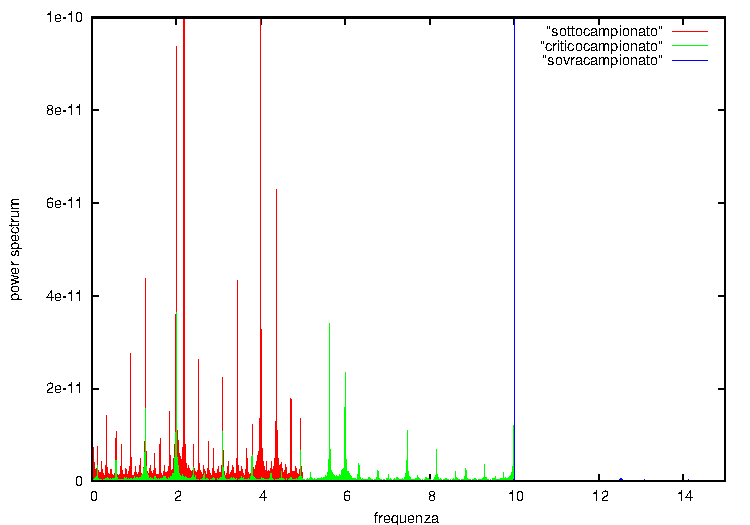
\includegraphics[width=10cm,keepaspectratio]{picture/confronto_aliasing}
\centering
\end{figure}

Come si può vedere dalla figura \ref{fig:aliasing}, per effetto del sottocampionamento tutte le componenti del segnale a frequenza maggiore di quella critica vengono ridistribuite nel intervallo $(-f_{c} , f_{c} )$.


\subsection{Trasformata come Filtro}

Sfruttanto il limite in frequenza imposto dalla frequenza critica per funzioni samplate, si può costruire un filtro passa basso.

L'idea è quella di determinare le frequenze principale dello spettro di una funzione ( una sinusoide a cui viene aggiunto un rumore bianco casuale) e da quelle ricostruire la funzione originale.
Per farlo si costruisce un algoritmo che a partire da un sampling di h(t) applica la trasformata discreta e successivamente l'anti trasformata, ricostruendo il segnale a partire dalle sue componenti di fourier a frequenza più bassa.
\begin{figure}[!h]
\caption{Filtro Passa - Basso}
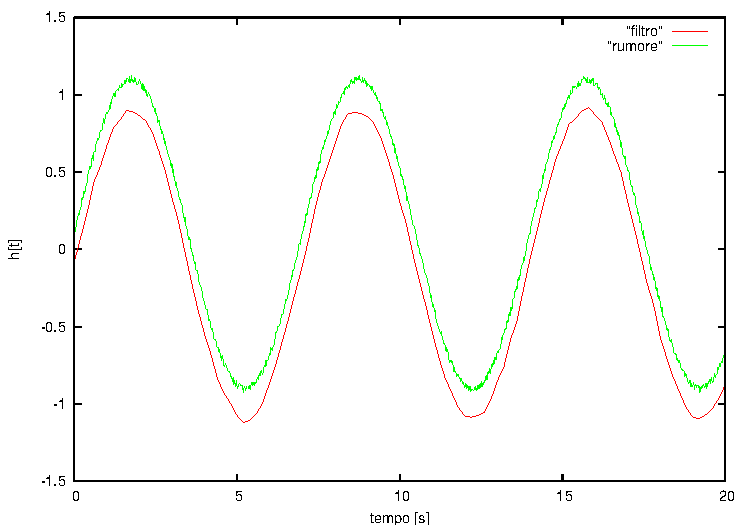
\includegraphics[width=10cm,keepaspectratio]{picture/filtrazione}
\centering
\label{fig:filtrazione}
\end{figure}

Dalla figura \ref{fig:filtrazione} è chiaro come il segnale trasformato due volte risulti maggiormente regolare, i termini spettrali che contengono l'informazione sul "rumore bianco" si trovano tutti a frequenze molto alte.

\subsection{Analisi Spettrale del Pendolo Caotico}

Prendendo in considerazione le soluzioni numeriche del equazione differenziale del pendolo Caotico ( con $l/g = 1$)

	\begin{equation}
\ddot{\theta}  = \qquad a\cos(\omega_{D} t) - \sin(\theta) -b \dot{\theta}
	\end{equation}

visto nella Relazione 4 è possibile, tramite lo studio dello spettro della soluzione , determinare delle componenti periodiche principali.

Le zone maggiormente piccate nello sviluppo di Fourier della funzione $\omega(t)$, velocità angolare in funzione del tempo, indicano la presenza di componenti periodiche principali.

In generale una funzione $h(t)$ che presenta una trasformata di Fourier discreta non potrà che essere periodica, il cui periodo è l'inverso del minimo comune multiplo di tutte le frequenze dello spettro.

Nelle configurazioni pseudocaotiche ci si aspetta una trasformata continua su un intero intervallo di frequenze, si può utilizzare lo sviluppo spettrale come criterio per identificare le regioni di caoticità


In tutti i casi considerati le condizioni iniziali sono fissate a $\theta_{0} = \pi / 2 \qquad \omega_{0} = 0$, le soluzioni sono campionate in $N = 131072$ punti ad intervalli di $\Delta = 0,05 s$, ciò implica un errore sul valore delle frequenze dello sviluppo spettrale di: 
$$ \delta f = \dfrac{1}{N \Delta} = \pm 0,000152588 .$$

Il numero di punti rende necessario l'utilazzo del algoritmo di Trasformata Rapida.

\section{Risultati}
\paragraph{Confronto tra diversi Pendoli}

Per prima cosa si possono confrontare la soluzione della velocità angolare per il pendolo in 3 configurazioni fondamentali:
	\begin{itemize}
	\item[-] Pendolo linearizzato : $[ a = 0 \, ;\, b = 0 \, ;\, sin(x) \simeq x ]$ da come risultato la soluzione valida per piccole oscillazioni.

Si attende una soluzione sinusoidale di periodo $T = 2 \pi \sqrt{l/g}\, \Rightarrow \, f = 1/T = 0.1592 Hz$.
	
\item[-] Pendolo semplice : $[ a = 0 \, ;\, b = 0 ]$.

Si attende una soluzione periodica di periodo minore del caso linearizzato e tendendente ad esso per $\theta_{0}$ piccolo.

\item[-] Pendolo Non Lineare ( o Caotico): $[ a = 0.9 \, ;\, \omega_{0} = 2/3 \, ;\, b = 0.5 ]$.

Pendolo completo di tutte le forze in una configurazione non caotica. Frequenza della forzante: $$f_{D} = \omega_{0}/(2 \pi) \, = \,0.1061$$ 
	\end{itemize} 

Si ottiene la figura spettrale \ref{fig:spettro_pendoli} :

\begin{figure}[!h]
\caption{Trasformata Pendoli}
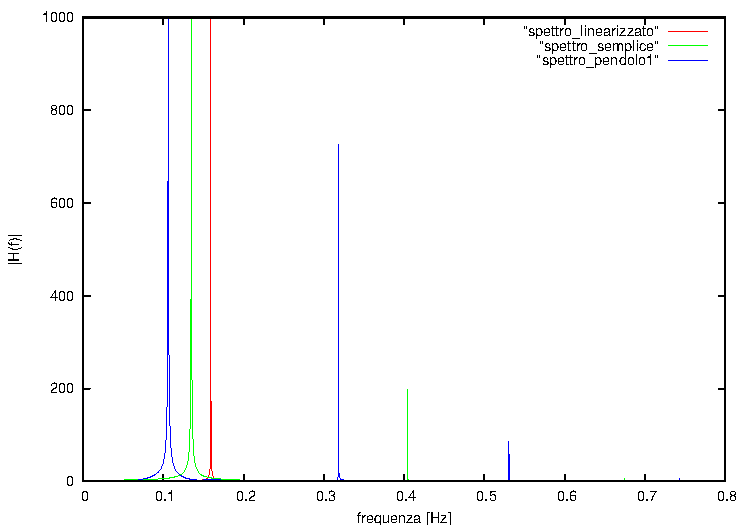
\includegraphics[width=10cm,keepaspectratio]{picture/spettro_pendoli}
\centering
\label{fig:spettro_pendoli}
\end{figure}

con i seguenti "picchi":

\begin{displaymath}
\centering
\begin{array}{|c|c|c|}
\hline
\textrm{pendolo} & \textrm{picco principale [Hz]} & \textrm{picchi secondari [Hz]} \\
\hline
\hline
Linearizzato &  0.1592	&  \\
\hline
Semplice &  0.1349	&	0.4045	\qquad 0.6741  \\
\hline
Non Lineare &  0.1061	&	0.3183	\qquad 0.5306 \qquad 0.7428 \\
\hline
\end{array}
\end{displaymath}

Come atteso, la soluzione del pendolo linearizzato è una sinusode il cui sviluppo spettrale è una $\delta$ centrata alla frequenza prevista mentre la soluzione per il pendolo non lineare presenta il picco più pronunciato alla frequenza della forzante: $$f_{0} = \frac{\omega_{0}}{2 \pi} = 1 / 3\pi \simeq 0.1061 \, \, .$$

In tutti i casi le soluzioni sono periodiche, lo si evince dallo spettro completamente discreto, presentano una frequenza dominante e nei casi del pendolo semplice e non lineare anche dei picchi a frequenze secondarie di intensità molto inferiore alla prima.

Nel caso del pendolo Non Lineare il primo picco corrisponde alla frequenza fondamentale, i picchi successivi sono a frequenza che è un multiplo intero della frequenza principale: 3,5,7; si conclude che è il primo picco a determinare il periodo della soluzione.

Le soluzioni presentano picchi alle seguenti frequenze
\begin{displaymath}
\centering
\begin{array}{|c|c|c|}
\hline
\textrm{pendolo} & \textrm{frequenza fondamentale} & \\
\hline
\hline
1 &  0.1592	&  \\
\hline
2 &  0.1349	&	0.4045	\qquad 0.6741  \\
\hline
3 &  0.1061	&	0.3183	\qquad 0.5306 \qquad 0.7428 \\
\hline
4 &  0.1061	&	0.3183	\qquad 0.5306 \qquad 0.7428 \\
\hline

\end{array}
\end{displaymath}


\clearpage
\paragraph{Confronto tra diversi pendoli Caotici}

Confrontando ora lo sviluppo spettarale della soluzione $\omega(t)$ per un pendolo non lineare con forzante di differente intensità: 

	\begin{itemize}
	\item[-] Pendolo 1 : $[ a = 0.9 \, ;\, \omega_{0} = 2/3 \, ;\, b = 0.5 ]$. Soluzione periodica alla stessa frequenza della forzante
	\item[-] Pendolo 2 : $[ a = 1.07 \, ;\, \omega_{0} = 2/3 \, ;\, b = 0.5 ]$. Soluzione periodica a frequenza dimezzata.
	\item[-] Pendolo 3 : $[ a = 1.47 \, ;\, \omega_{0} = 2/3 \, ;\, b = 0.5 ]$. Soluzione periodica a frequenza  ulteriormente dimezzata.
	\item[-] Pendolo 4 : $[ a = 1.5 \, ;\, \omega_{0} = 2/3 \, ;\, b = 0.5 ]$. Soluzione caotica.
	\end{itemize} 

\begin{figure}[!h]
\caption{Confronto Spettro Pendoli Non Lineari}
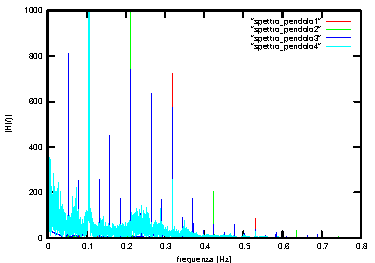
\includegraphics[width=10cm,keepaspectratio]{picture/spettro_tutto}
\centering
\label{fig:caotici}
\end{figure}

Dai grafici \ref{fig:caotici} e \ref{fig:quadro} emerge che il sistema presenta in ogni caso , anche nella configurazione caotica 4, il picco più marcato alla frequenza di oscillazione della forzante.

A differenza dei primi 3 pendoli che possiedono uno spettro chiaramente discreto (vedere tabella successiva), il pendolo 4, pur presentando un evidente picco alla frequenza della forzante, ha dei termini spettrali sparsi in modo continuo su tutte le frequenza più basse.

Apparentemente è come se i termini discreti dei pendoli precendenti tendano a moltiplicarsi tanto ( il periodo si raddoppia), fino al continuo, al tendere del parametro di intensità $a$ al valore $1,5$.

In sostanza c'è un accorto tra la natura continua dello spettro e la pseudocaoticità della soluzione; questo è quantomeno ragionevole, non ci si può aspettare una struttura periodica da una soluzione che dovrebbe in qualche modo inglobare la natura non regolare del caos.


\begin{minipage}{.42\textwidth}
\begin{displaymath}
\begin{array}{|c|c|c|l}
\hline
\textrm{Pendolo 1} & \textrm{Pendolo 2}  & \textrm{Pendolo 3}  \\
\hline
\hline
 0,1060 & 0,0531 & 0,0000 \\
 0,3183 & 0,1060 & 0,0266 \\
 0,5305 & 0,1541 & 0,0531 \\
 0,7428 & 0,2123 & 0,0797 \\
   & 0,2652 & 0,1060 \\
   & 0,3183 & 0,1326 \\
   & 0,3714 & 0,1591 \\
   & 0,4243 & 0,1857 \\
   & 0,4774 & 0,2123 \\
   & 0,5305 & 0,2388 \\
   & 0,5835 & 0,2652 \\
   & 0,6366 & 0,2917 \\
   &   & 0,3183 \\
   &   & 0,3449 \\
   &   & 0,3714 \\
   &   & 0,3979 \\
   &   & 0,4243 \\
   &   & 0,4509 \\
   &   & 0,4774 \\
   &   & 0,5040 \\
   &   & 0,5305 \\
   &   & 0,5571 \\
   &   & 0,5835 \\
\hline
\end{array}
\end{displaymath}
\end{minipage}
\begin{minipage}{.60\textwidth}

I primi 3 pendoli presentano un numero discreto di picchi equidistanti l'uno dall'altro.
Uno sviluppo spettrale discreto implica la periodicità della soluzione, in tutti i casi si nota l'esistenza di una frequenza fondamentale $\nu_{0}$ di cui i picchi successivi sono un semplice multiplo intero:

 - Pendolo1 : $\Delta\nu \sim 0,221 Hz \qquad \nu_{0}\sim 0,106 Hz$ .

 - Pendolo2 : $\Delta\nu \sim 0,053 Hz  \qquad \nu_{0}\sim 0,053 Hz$ .

 - Pendolo3 : $\Delta\nu \sim 0,027 Hz  \qquad \nu_{0}\sim 0,027 Hz$ .

Di conseguenza il periodo delle soluzioni è l'inverso della frequenza fondamentale da questo si evidenzia il raddoppiamento del periodo nel passaggio da una configurazione alla succesiva.
\end{minipage}



\begin{sidewaysfigure}[!h]
\caption{Trasformata Pendoli Non Lineari}
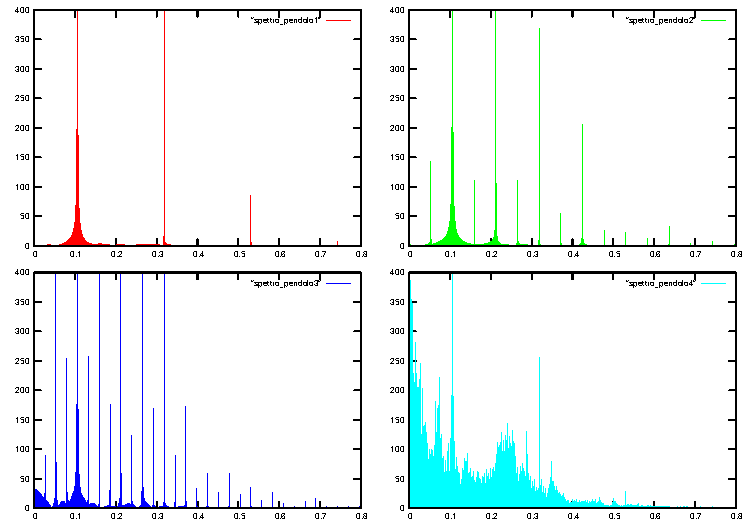
\includegraphics[width=24cm,keepaspectratio]{picture/quadro}
\centering
\label{fig:quadro}
\end{sidewaysfigure}



\clearpage
\begin{thebibliography}{99}
\bibitem{recipe}\emph{Numerical recipes in C++}
\bibitem{knuth}Knuth D. \emph{The Art of Computer Programming}
\bibitem{hilde}Hildebrand F. \emph{Introduction to Numerical Analysis}, 2nd.ed.
\end{thebibliography}
\end{document}




